\documentclass[letterpaper,9pt,twocolumn,twoside,]{pinp}

%% Some pieces required from the pandoc template
\providecommand{\tightlist}{%
  \setlength{\itemsep}{0pt}\setlength{\parskip}{0pt}}

% Use the lineno option to display guide line numbers if required.
% Note that the use of elements such as single-column equations
% may affect the guide line number alignment.

\usepackage[T1]{fontenc}
\usepackage[utf8]{inputenc}

% pinp change: the geometry package layout settings need to be set here, not in pinp.cls
\geometry{layoutsize={0.95588\paperwidth,0.98864\paperheight},%
  layouthoffset=0.02206\paperwidth, layoutvoffset=0.00568\paperheight}

\definecolor{pinpblue}{HTML}{185FAF}  % imagecolorpicker on blue for new R logo
\definecolor{pnasbluetext}{RGB}{101,0,0} %



\title{Multiple Regression Analysis of Body Fat Percent based on Siri
Equation}

\author[a]{Dawei Yun}
\author[a]{Tianshuai Gao}
\author[a]{Sophie Su}
\author[a]{Haohao Li}

  \affil[a]{DATA2002 RE03E1 USYD}

\setcounter{secnumdepth}{0}

% Please give the surname of the lead author for the running footer
\leadauthor{}

% Keywords are not mandatory, but authors are strongly encouraged to provide them. If provided, please include two to five keywords, separated by the pipe symbol, e.g:
 \keywords{  Siri Equation |  Linear regression |  Model Selection  }  

\begin{abstract}
In this report, we will demonstrate that factors other than body density
may be utilized to predict body fat percentage based on Siri equation
``\% Body Fat = (495 / Body Density)--450'' (Siri 1961). Some predictive
linear models were built using the research of correlations between the
target variable, body fat percentage, and other independent variables
that retained certain linearity. Model selection is implemented using a
variety of techniques, including assumption test, forward and backward
method selection, and 10-fold cross-validation. The conclusion is that
body fat percentage and body density, together with age and abdomen as
other independent variables, can establish a linear regression
\end{abstract}

\dates{This version was compiled on \today} 


% initially we use doi so keep for backwards compatibility
% new name is doi_footer
\doifooter{\url{https://github.sydney.edu.au/FESU3631/RE03-E1}}


\begin{document}

% Optional adjustment to line up main text (after abstract) of first page with line numbers, when using both lineno and twocolumn options.
% You should only change this length when you've finalised the article contents.
\verticaladjustment{-2pt}

\maketitle
\thispagestyle{firststyle}
\ifthenelse{\boolean{shortarticle}}{\ifthenelse{\boolean{singlecolumn}}{\abscontentformatted}{\abscontent}}{}

% If your first paragraph (i.e. with the \dropcap) contains a list environment (quote, quotation, theorem, definition, enumerate, itemize...), the line after the list may have some extra indentation. If this is the case, add \parshape=0 to the end of the list environment.


\hypertarget{introduction}{%
\subsection{Introduction}\label{introduction}}

Sociologists, biologists, and psychologists often study human
performance in and across multiple characteristics to identify and
analyze the underlying manifestations. The percentage of body fat is one
of the key values that reflected the health and fitness of human beings.
However, the accurate measurement of body fat percentage is difficult to
handle and expensive. Hence, the application of calculations between
other easily measurable attributes might be more effective. According to
the Siri equation, body fat percentage could be calculated by body
density directly. In this report, we will build and evaluate the
regression models to find out whether the model could predict the target
variable effectively and efficiently with certain attributes. People who
are interested in predictive methods, human performance study, and
fitness might be the stakeholders.

\hypertarget{data-set}{%
\subsection{Data set}\label{data-set}}

The data set was gathered by DASL (The Data and Story Library), an
archive of hundreds of data files that provide a platform for statistics
and data science study for students and teachers. The original source of
this data set is BYU Human Performance Research Center. There were many
methods used to collect and describe data including multiple regression,
display of quantitative variables, hypothesis tests, partial regression
plots, confidence intervals for proportions, sampling distribution, and
so on. The dataset included 250 numerical observations within 16
variables. There were no missing or zero values and one outlier. The
target variable is the percentage of body fat and other variables are
described as physical characteristics involving density, age, weight,
neck, chest, abdomen, waist, hip, thigh, knee, ankle, bicep, forearm,
and wrist. To estimate the body density, the technique underwater would
be used. The calculation of body volume is equal to the loss of weight
in water with the temperature correction for the water's density, which
is complicated. There was an unwanted outlier in the body fat percentage
variable.

\hypertarget{analysis}{%
\subsection{Analysis}\label{analysis}}

\hypertarget{dependent-variable-selection}{%
\subsubsection{Dependent variable
selection}\label{dependent-variable-selection}}

Before choosing a model, we must choose the appropriate independent
variable (x-value) and how many independent variables. The first is to
contrast correlation coefficient plots to determine our independent
variables, but it is challenging to select the correct variables from
the naked eye. Thus, we decided to use forward and backward methods.

\hypertarget{forward-backward-elimination}{%
\subsubsection{Forward \& Backward
Elimination}\label{forward-backward-elimination}}

The specific operation steps: First, fit the model with the independent
variable with the most significant correlation coefficient with the
dependent variable y, carry out the significance test of the regression
coefficient, and decide whether to introduce the independent variable
into the model. (The value with the symbol *) By eliminating forward and
backward, we derive the best three values for abdomen, density and age
as dependent variables.

\begin{center}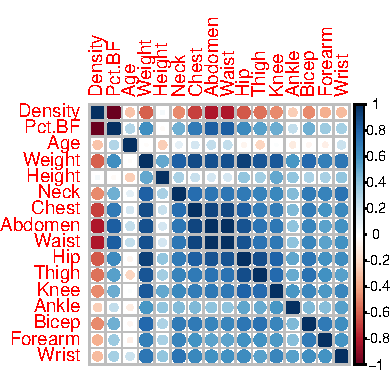
\includegraphics{DATA2002-RE03E1_files/figure-latex/unnamed-chunk-4-1} \end{center}

\hypertarget{model-selection}{%
\subsubsection{Model selection}\label{model-selection}}

Many models can predict our dependent variable, but we may not know
which is the most suitable. At first, we used the most basic linear
model to predict our PBF value by adding the three independent variables
of density, age, and abdomen to form a linear model to see if it is
suitable. Nevertheless, how do we go to see if it fits the modelling?

\hypertarget{adjusted-r-squared}{%
\subsubsection{Adjusted R-Squared}\label{adjusted-r-squared}}

\begin{figure}[hbt!]
  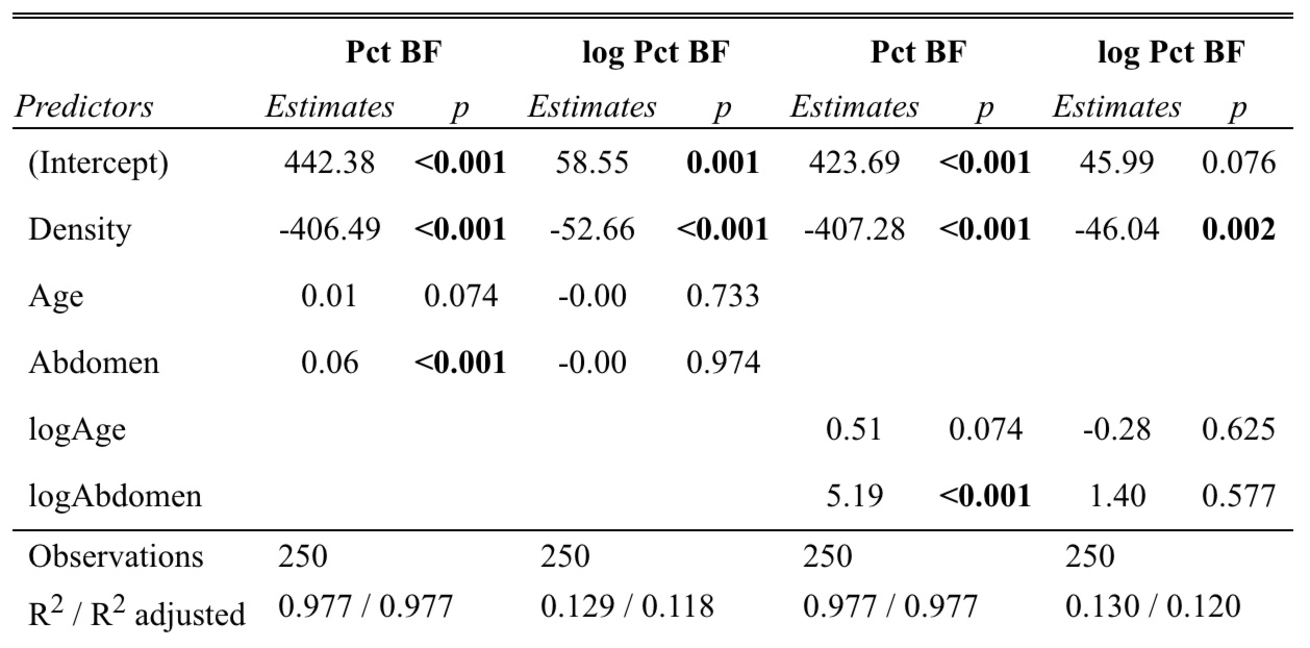
\includegraphics[width=3.43in, height=1.7in]{abc} 
\end{figure}

We can determine our model by comparing the size of the Adjusted
R-Squared in each model. R\^{}2 shows how good terms (data points) fit a
curve or line. Adjusted R\^{}2 indicates how well terms fit a curve or
line but adjusts for the number of terms in a model. That is, valid
variables added to the model will reduce the size of the R-squared,
while invalid variables will only reduce its size and fit. So we
performed several (Linear - Log, Log-linear, Log - Log) modelling to
compare the size of the r-squared to select our model. However, because
the model does not pass the assumption, we rejected the lowest two
Adjusted r-squared models. linear-log would be our final model.

\hypertarget{assumption-check}{%
\subsubsection{Assumption Check}\label{assumption-check}}

\begin{figure}[hbt!]
  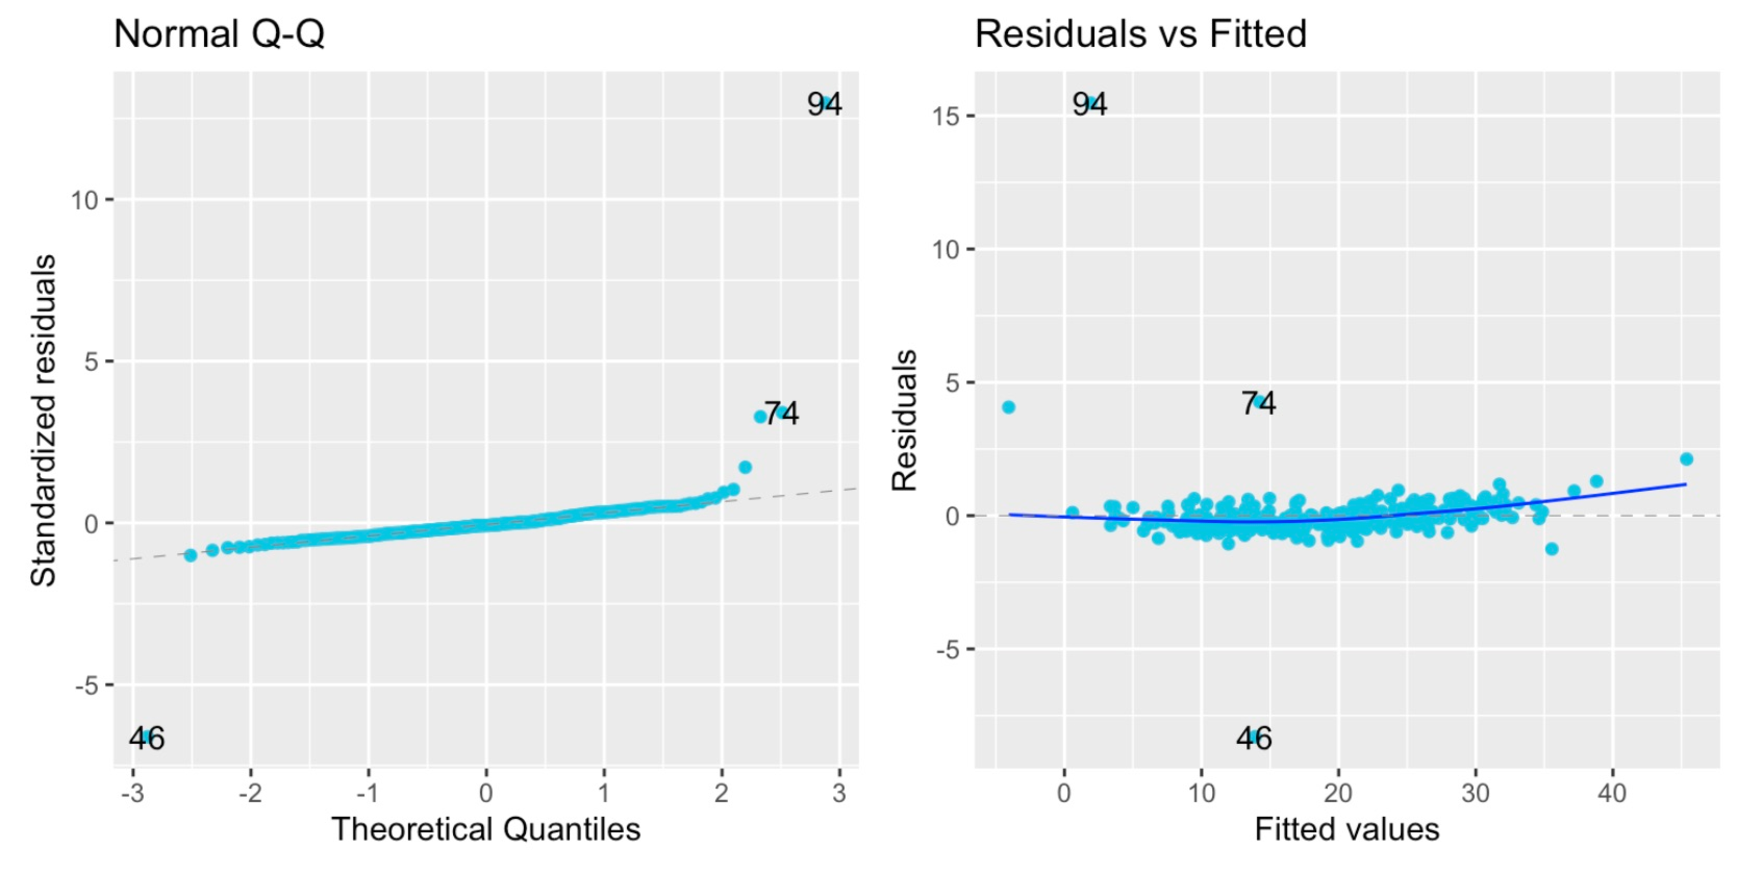
\includegraphics[width=3.2in, height=1.6in]{abcd} 
\end{figure}

\hypertarget{linearity}{%
\paragraph{Linearity}\label{linearity}}

On the residuals and the fit plot. In the figure, we can see a clear
pattern in the residual plot. And the pattern does not appear obvious
shape. This would indicate that there is a linear relationship between
the predictors and the outcome variable.

\hypertarget{independence}{%
\paragraph{Independence}\label{independence}}

From the source of the data set. We know that the variable in the data
set is not related to the other variables. Secondly, we used
Durbin-Watson test. The null hypothesis of the Durbin-Watson test says
that they are independent. Our P-value is 0.272, we will not be able to
reject the null hypothesis. This will provide us with enough evidence to
show that our independence assumption is satisfied!

\hypertarget{homoskedasticity}{%
\paragraph{Homoskedasticity}\label{homoskedasticity}}

On the residuals and fit plots, we can see the spread looks relatively
constant over the range of fitted values. And the residuals are
uniformly distributed. So, this assumption is valid.

\hypertarget{normality}{%
\paragraph{Normality}\label{normality}}

It can be seen from the Q-Q plot that most points are in a straight
line. Therefore, the assumption of normality of the residuals is well
satisfied.

\hypertarget{results}{%
\subsection{Results}\label{results}}

\begin{itemize}
\tightlist
\item
  Compare them to the observed values using the root mean square error:
\end{itemize}

\[RMSE = \sqrt( \frac{\sum_{i=1}^n (y_i - \hat{y_i})^2 }{n} )\]

\begin{itemize}
\tightlist
\item
  An alternative measure of performance, less influenced by outliers is
  the mean absolute error:
\end{itemize}

\[MAE = \frac{\sum_{i=1}^m |y_i - \hat{y_i}|}{m}\]

\begin{center}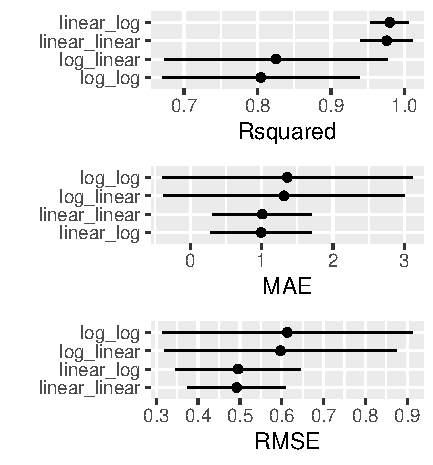
\includegraphics{DATA2002-RE03E1_files/figure-latex/unnamed-chunk-19-1} \end{center}

Linear-log Model has the biggest R-squared and smallest MAE and RMSE

\[Pct.BF = 423.7 - 407.3 \cdot Density + 0.5 \cdot \log(\overbrace{Age}) + 5.2 \cdot \log(\overbrace{Abdomen})\]

\begin{itemize}
\item
  A one year increase in Age results in a 0.5089\% change in Pct.BF on
  average, holding Density and Abdomen constant.
\item
  A one centimeter increase in Abdomen results in a 5.1896\% change in
  Pct.BF on average, holding Age and Density
\item
  A one unit decrease in Density results in a 407.2826 change in Pct.BF
  on average, holding Age and Abdomen constant
\end{itemize}

\hypertarget{discussion-and-conclusion}{%
\subsection{Discussion and Conclusion}\label{discussion-and-conclusion}}

\hypertarget{limitations}{%
\subsubsection{limitations}\label{limitations}}

The report explores the linear relationship between \textbf{Density} and
\textbf{Pct.BF} based on Siri equation.However the Siri equation is not
just a simple linear regression.

For selection bias, there are only male above 22-year-old observations
included which could not represent the whole population. The calculation
of bodyfat percentage highly depends on the density, which might be
considered as designed bias. Any human performance inferences are thus
limited.

\hypertarget{future-research}{%
\subsubsection{Future Research}\label{future-research}}

In the future, we need to use different linear regression models (Lasso
Regression, Ridge Regression) to improve the relationship between
density and Pct.BF

This report only discusses a simple linear model. More different Machine
Learning Model like K-Nearest Neighbors Model, Random Forest Model etc
should be considered. Comparisons of limitations and uncertainties about
the different Models is an important step that cannot to be ignored.

\hypertarget{conclusion}{%
\subsubsection{Conclusion}\label{conclusion}}

Body Density should be a factor which pay more attention to due to the
huge direct effect of body density on percent body fat.

With age, percent body fat will also increase gradually, but we can
effectively maintain a reasonable percent body fat by exercising the
abdominal muscles.

A healthy amount of body fat is necessary for the body to function
properly. While excess body fat is associated with an increased risk of
heart disease,too little body fat is just as dangerous.

\hypertarget{reference}{%
\section{Reference}\label{reference}}

Alboukadel Kassambara. 2020. ggpubr: `ggplot2' Based Publication Ready
Plots. R package version 0.4.0, URL
\url{https://CRAN.R-project.org/package=ggpubr}.

Barret Schloerke, Di Cook, Joseph Larmarange, Francois Briatte, Moritz
Marbach, Edwin Thoen, Amos Elberg, Ott Toomet, Jason Crowley, Heike
Hofmann and Hadley Wickham. 2022. GGally: Extension to 'ggplot2'. R
package version 2.1.2, URL
\url{https://CRAN.R-project.org/package=GGally}.

Daniel Ludecke. 2022. sjPlot: Data Visualization for Statistics in
Social Science. R package version 2.8.11, URL
\url{https://CRAN.R-project.org/package=sjPlot}.

Dodge, Y. 2008. The Concise Encyclopedia of Statistics. Switzerland:
Springer.

Everitt, B. S., and Skrondal, A. 2010. The Cambridge Dictionary of
Statistics. London: Cambridge University Press.

Gonick, L. 1993. The Cartoon Guide to Statistics. New York:
HarperPerennial.

Hadley Wickham and RStudio. 2022. tidyverse: Easily Install and Load the
`Tidyverse'. R package version 1.3.2 , URL
\url{https://CRAN.R-project.org/package=tidyverse}.

Hadley Wickham, Romain Francois, Lionel Henry and Kirill Muller. 2022.
dplyr: A Grammar of Data Manipulation. R package version 1.0.10.
\url{https://CRAN.R-} project.org/package=dplyr.

JJ Allaire and others.2022. rticles: Article Formats for R Markdown. R
package version 0.24, URL
\url{https://CRAN.R-project.org/package=rticles}.

John Fox and others. 2022. car: Companion to Applied Regression. R
package version 3.1-1, URL \url{https://CRAN.R-project.org/package=car}.

Karl W Broman, Michael Bostock and other jQuery contributors. 2022.
qtlcharts: Interactive Graphics for QTL Experiments. R package version
0.16, URL \url{https://CRAN.R-project.org/package=qtlcharts}.

Max Kuhn and others. 2022. caret: Classification and Regression
Training. R package version 6.0-93, URL
\url{https://CRAN.R-project.org/package=caret}.

Masaaki Horikoshi, Yuan Tang, Austin Dickey, Matthias Grenié, Ryan
Thompson, Luciano Selzer, Dario Strbenac, Kirill Voronin and Damir
Pulatov. 2022. ggfortify: Data Visualization Tools for Statistical
Analysis Results. R package version 0.4.14, URL
\url{https://CRAN.R-project.org/package=ggfortify}.

Philippe Grosjean, Frederic Ibanez, Michele Etienne. 2018. pastecs:
Package for Analysis of Space-Time Ecological Series. R package version
1.3.21, URL \url{https://CRAN.R-project.org/package=pastecs}.

Siri, W. E. 1961. Body composition from fluid space and density. In J.
Brozek \& A. Hanschel (Eds.), Techniques for measuring body composition
(pp.~223-244). Washington, DC: National Academy of Science.

Taiyun Wei, Viliam Simko, Michael Levy , Yihui Xie, Yan Jin, Jeff Zemla,
Moritz Freidank, Jun Cai, Tomas Protivinsky. 2021. corrplot:
Visualization of a Correlation Matrix. R package version 0.92, URL
\url{https://CRAN.R-project.org/package=corrplot}.

Wood, R. 2008. Siri equation. Topend Sports. Available at:
\url{https://www.topendsports.com/testing/siri-equation.htm} (Accessed:
November 5, 2022).

Yihui Xie and others. 2022. knitr: A General-Purpose Package for Dynamic
Report Generation in R. R package version 1.40 , URL
\url{https://CRAN.R-project.org/package=knitr}.

%\showmatmethods

\pnasbreak 




\end{document}
